%Adaptado de
%=========
%% bare_jrnl.tex
%% V1.4b
%% 2015/08/26
%% by Michael Shell
%=======
%Definición del tipo de documento
\documentclass[journal]{IEEEtran}
%Paquetes que se usarán
%Paquete de codificación
\usepackage[utf8]{inputenc}
%Paquete de idioma
\usepackage[spanish]{babel}
%Paquete para manejo de URLs.
\usepackage{hyperref}
%Paquete para manejo general de imágenes
\usepackage{graphicx}
%También se puede(n) indicar la ubicación de algunas carpetas que contienen diversos documentos, imágenes, código, bibliografía, etc.
%\addbibresource{mybibliography.bib}
\graphicspath{{./Imagenes/}}

\begin{document}
\title{Informe}

\author{Wilmer~Banquez,~\IEEEmembership{}
        David~Arango,~\IEEEmembership{}
        y~Juliana~Martínez~\IEEEmembership{}
}

% The paper headers
\markboth{Informática II - 2022}{}

% make the title area
\maketitle

%%\begin{abstract}
%%El circuito 74HC595 
%%\end{abstract}

% Note that keywords are not normally used for peerreview papers.
\begin{IEEEkeywords}
Arduino, Integrado 74HC595, etc.
\end{IEEEkeywords}

\section{Introducción}

\IEEEPARstart{E}{l} chip 74HC595 es un circuito impresor, concretamente es un registro de desplazamiento de 16 pines que sirve para convertir datos de serie a paralelo de una forma eficaz y sencilla. En el siguiente informe se encuentran dos ejemplos de cómo utilizar dicho circuito, después detallamos la utilidad que podemos darle para solucionar la implementación del sistema de encriptación en los dos arduinos. Por último se plantea un posible diseño.\\
% You must have at least 2 lines in the paragraph with the drop letter
% (should never be an issue)"Si algo puede ir mal, saldrá mal y de la peor forma, siempre".

\section{Circuito integrado 74HC595}
Como primera medida, se propuso el ejercicio de representar números binarios de forma manual usando una protoboard, un suministro de energía, un switch deslizante, dos pulsadores, luces led, el circuito integrado 74HC595, resistencias y cables. La primera etapa del ejercicio se basa en la estructuración general de los cables para efectuar la conexión entre el circuito integrado, los pulsadores, el switch y demás componentes. El funcionamiento constaba de un switch deslizante (data) que dependiendo del estado en el que se encontrara (encendido o apagado) comunicaba cierta información (1 o 0), a continuación el primero de los pulsadores recibe esta información las veces que fuera accionado. Por último, el segundo pulsador toma el registro y lo expone a la salida en este caso reflejándolo en las led.\\
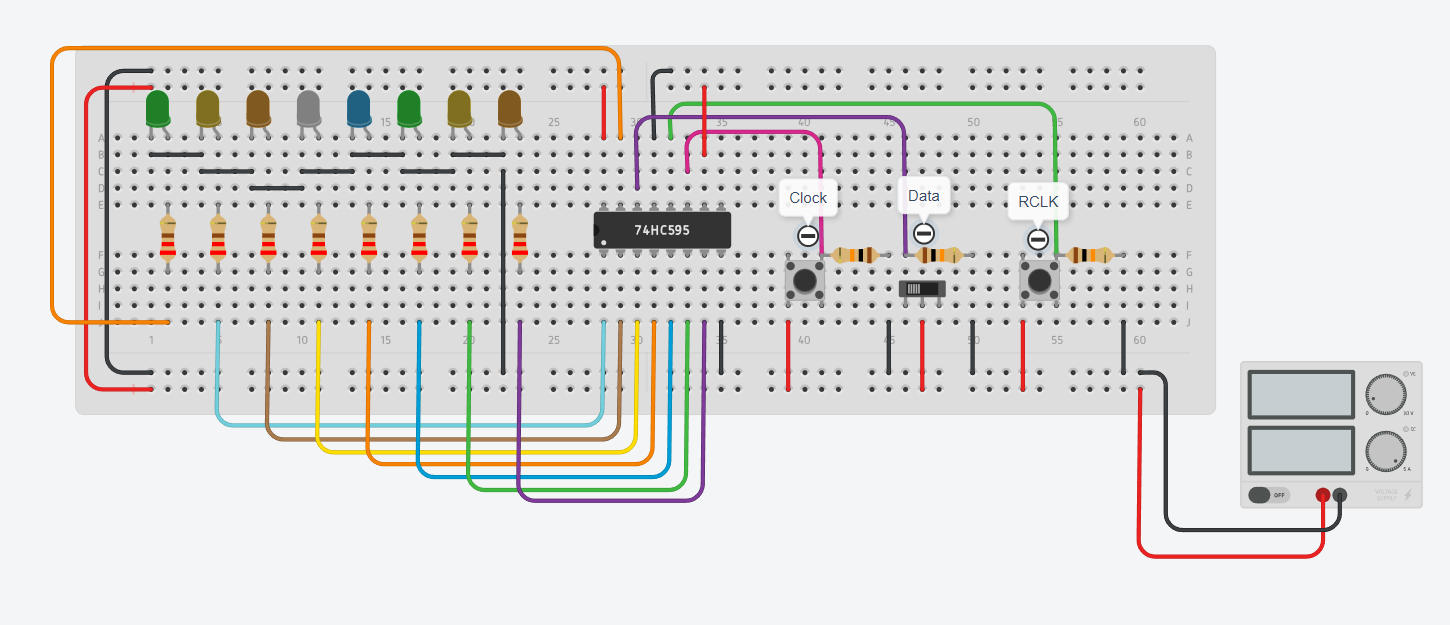
\includegraphics[width=9cm]{Imagenes/image (1).png}\\
\url{https://www.tinkercad.com/things/fdPmct90xWs}.\\
En el segundo ejemplo aplicado se utilizaron luces leds, resistencias, un arduino, una protoboard, cables y obviamente el circuito integrado 74HC595. El objetivo a cumplir era convertir un caracter ingresado por el usuario a codigo binario, principalmente mediante hardware. Una vez más se llevaron a cabo todos los cableados necesarios para que la conexión entre las componentes fuera óptima.\\
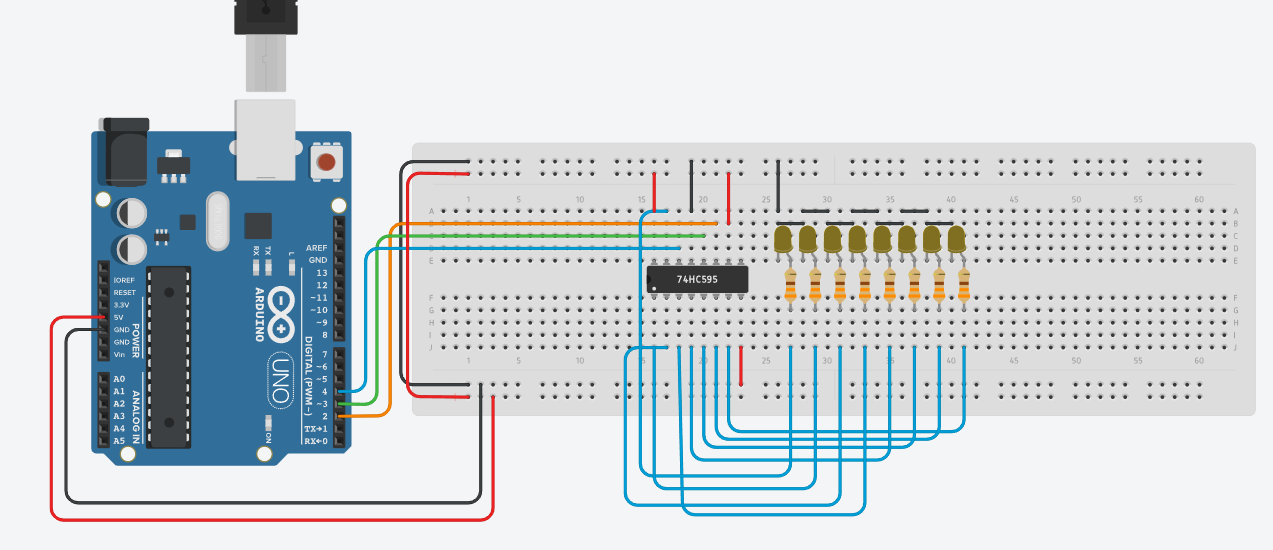
\includegraphics[width=9cm]{Imagenes/image.png}
\url{https://www.tinkercad.com/things/ajHYnGZvnA2}.\\
A continuación se usaron las resistencias y las LED para representar la conversión del caracter a código binario realizada por el propio circuito. En lo que respecta al código, se tomaron medidas específicas como restringir el rango de los caracteres ya que si éste se encontraba fuera de 0 y 255 no correspondería a código ASCII lo cual arrojaría un error.
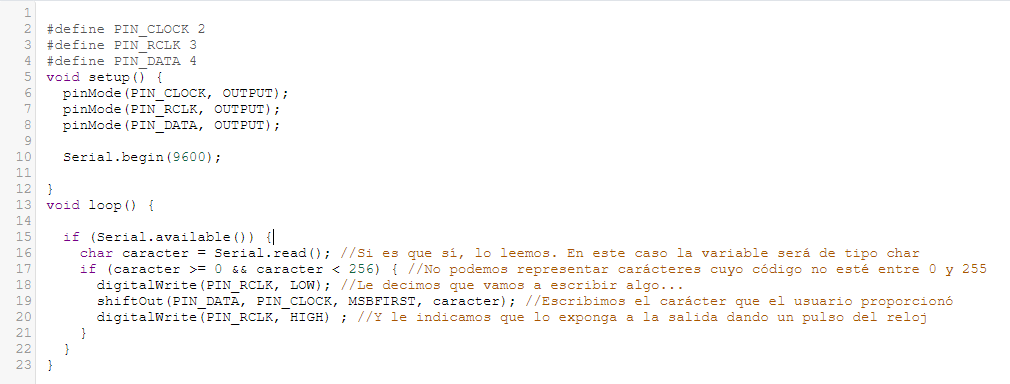
\includegraphics[width=9cm]{Imagenes/image (2).png}
\section{Utilidad}
Sabiendo que el circuito integrado paraleliza los datos que recibe, éste facilitaría la labor de desencriptar la información mediante el método que se requiera.\\
\section{Conclusiones}
¿Qué sucede con las tablas?\\
En la documentación se encuentra el código, explicado y con ejemplos, para esto.
\ifCLASSOPTIONcaptionsoff
  \newpage
\fi


\begin{thebibliography}{1}

\bibitem{IEEEhowto:kopka}
H.~Kopka and P.~W. Daly, \emph{A Guide to \LaTeX}, 3rd~ed.\hskip 1em plus
  0.5em minus 0.4em\relax Harlow, England: Addison-Wesley, 1999.

\end{thebibliography}
\end{document}

